\begin{frame}{Three activities for descriptive statistics}
\begin{enumerate}
\item \textbf{2A: Reading data and graphs}\\Measurement, denominators, missing values and graphical choices.
\item \textbf{2B: Centre and variability}\\Mean, median, quantiles, variance and relative spread.
\item \textbf{2C: Heterogeneity and indices}\\Categorical diversity, standardisation and interpretation.
\end{enumerate}
\prompt{Predict, explore, explain. Each activity ends with a decision task and a quiz.}
\end{frame}


\begin{frame}{E-tivity 2A: Reading data and graphs}
\Large Reading data and graphs\par\vspace{5mm}
\normalsize Complete the matching activity in the descriptive learning path.\par
\href{https://silviasaliniunimi.github.io/data-analysis-tax-compliance/02a-graphs.html}{Open E-tivity 2A}\par

\end{frame}

\begin{frame}{Measurement determines meaningful operations}
\small\begin{tabular}{>{\raggedright\arraybackslash}p{.19\textwidth}>{\raggedright\arraybackslash}p{.32\textwidth}>{\raggedright\arraybackslash}p{.38\textwidth}}\toprule
\textbf{Scale} & \textbf{Example} & \textbf{Meaningful operations}\\\midrule
Nominal & Sector, filing channel & Equality, counts and proportions\\[3mm]
Ordinal & Low / medium / high risk band & Order, counts and cumulative proportions\\[3mm]
Interval & Temperature in Celsius & Differences; ratios depend on the chosen zero\\[3mm]
Ratio & Turnover, elapsed time & Differences and ratios, with a meaningful zero\\\bottomrule
\end{tabular}\par
\par\vspace{3mm}\normalsize Numerical codes do not change the scale. A firm ID is a label.\\
Discrete/continuous describes possible numerical values, not measurement scale.
\end{frame}

\begin{frame}{Validity and reliability}
\textbf{Validity: does the variable capture the intended concept?}\\
Filing delay measures timeliness. It does not capture every aspect of tax compliance.
\par\vspace{4mm}
\textbf{Reliability: is the measurement consistent?}\\
The same coding rule applied to the same records should produce consistent results.
\par\vspace{4mm}
A consistently recorded variable can still be a poor measure of the intended concept.
\prompt{Which definition and data checks would you require before comparing offices?}
\end{frame}

\begin{frame}{A proportion needs a denominator}
If $n_j$ observations belong to category $j$, the relative frequency is
\[p_j=\frac{n_j}{n},\qquad \sum_j p_j=1.\]
In the data: 18 online filings out of 24, so $p=0.75$.\\
Delay is observed for 22 firms. Of these, 18 have a positive delay:
\[18/22=81.8\% \quad\text{among records with known delay}.\]
The late proportion among all 24 lies between $18/24$ and $20/24$, if each missing value could be either on time or late.
\end{frame}

\begin{frame}{Revenue amounts and payment ratios}
\small
\begin{tabular}{lrrr}\toprule
District & Assessed amount & Matched payments & Payment ratio\\\midrule
A & 160 & 120 & $75\%$\\
B & 40 & 36 & $90\%$\\\midrule
Combined & 200 & 156 & $78\%$\\\bottomrule
\end{tabular}\par\vspace{3mm}
The combined ratio is $156/200$, not $(75\%+90\%)/2$.\\
Weight the district ratios by their assessed amounts:
\[\frac{160}{200}\,75\%+\frac{40}{200}\,90\%=78\%.\]
\textbf{Interpretation:} payments relative to recorded assessments.\\
This does not reveal obligations missing from those assessments.
\source{Synthetic district example from E-tivity 1, separate from the 24-firm dataset. Same reference period and payment date; monetary values in arbitrary units.}
\end{frame}

\begin{frame}{Missingness changes the interpretation}
\begin{itemize}
\item A missing value can mean unrecorded, unavailable or not applicable. Check its definition.
\item Report how many observations enter each calculation.
\item Replacing missing values by zero changes the variable and can distort its distribution.
\item Describing complete records does not establish that they represent the missing records.
\end{itemize}
\end{frame}

\begin{frame}{Different graphs answer different questions}
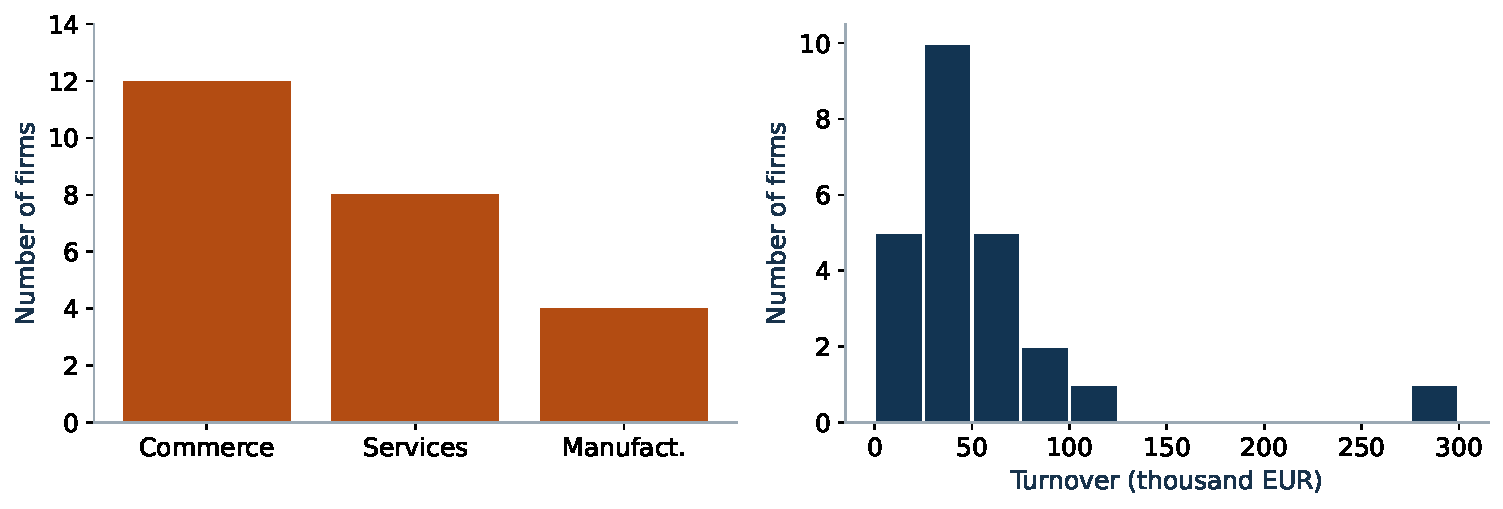
\includegraphics[width=\textwidth]{figures/distributions.pdf}
Bars show categories. Histograms group numerical values into intervals.\\
For a histogram, bin boundaries are part of the presentation.
\end{frame}

\begin{frame}{Common sources of misleading graphs}
\small
\begin{tabular}{>{\raggedright\arraybackslash}p{.34\textwidth}>{\raggedright\arraybackslash}p{.55\textwidth}}\toprule
\textbf{Display choice} & \textbf{What to check}\\\midrule
Truncated bar baseline & Bar length normally requires a zero baseline.\\[3mm]
Unordered ordinal categories & Keep the natural order of the scale.\\[3mm]
Numerical values used as labels & Preserve numerical distances, including gaps.\\[3mm]
Counts compared across groups & State the denominator when the question concerns rates.\\[3mm]
Pie chart for multiple responses & Overlapping responses are not parts of one whole.\\\bottomrule
\end{tabular}\par\vspace{3mm}
In a survey of 100 taxpayers, 65 use online help, 45 telephone help and 30 a service desk. Bars can show these percentages; a pie cannot represent their overlap.
\source{Adapted from the supplied Misleading Graphs e-tivity. Numerical scenario is illustrative.}
\end{frame}

\begin{frame}{Unequal bins require density on the vertical axis}
Consider the bins $[0,50)$, $[50,100)$, $[100,200)$ and $[200,400]$.
\begin{center}\begin{tabular}{lrrr}\toprule
Interval & Count & Width & Count / width\\\midrule
0--50 & 15 & 50 & 0.30\\
50--100 & 7 & 50 & 0.14\\
100--200 & 1 & 100 & 0.01\\
200--400 & 1 & 200 & 0.005\\\bottomrule
\end{tabular}\par\end{center}
Histogram \textbf{area} represents frequency. With unequal widths, the modal interval has the greatest density. For relative density, also divide by $n$.
\end{frame}

\begin{frame}{E-tivity 2B: Centre and variability}
\Large Centre and variability\par\vspace{5mm}
\normalsize Complete the matching activity in the descriptive learning path.\par
\href{https://silviasaliniunimi.github.io/data-analysis-tax-compliance/02b-centre-spread.html}{Open E-tivity 2B}\par

\end{frame}

\begin{frame}{Mode, median and mean describe different features}
\begin{tabular}{>{\raggedright\arraybackslash}p{.16\textwidth}>{\raggedright\arraybackslash}p{.73\textwidth}}\toprule
Mode & Most frequent value or category. There may be ties.\\[3mm]
Median & Middle position after ordering. For even $n$, average the two central numerical values.\\[3mm]
Mean & Total divided by the number of observations: $\bar{x}=\frac1n\sum_i x_i$.\\\bottomrule
\end{tabular}\par
\par\vspace{3mm}Turnover in the synthetic data: mode 20, median 41, mean 56.75 thousand EUR.\\
For nominal categories, a numerical mean has no intrinsic meaning.
\end{frame}

\begin{frame}{The median with grouped observations}
\small
\begin{tabular}{lrr}\toprule
Processing time (hours) & Count & Cumulative count\\\midrule
$[0,12)$ & 8 & 8\\
$[12,24)$ & 15 & 23\\
$[24,36)$ & 12 & 35\\
$[36,48]$ & 5 & 40\\\bottomrule
\end{tabular}\par
The midpoint of the cumulative distribution lies in $[12,24)$.
\[\widehat{\mathrm{Median}}=12+\frac{20-8}{15}\times12=21.6\text{ hours}.\]
Linear interpolation assumes a uniform spread within the median interval. The exact raw-data median is unknown.
\source{Adapted from Measures of Location. The class midpoint 18 is not automatically the median.}
\end{frame}

\begin{frame}{Extreme values can move the mean substantially}
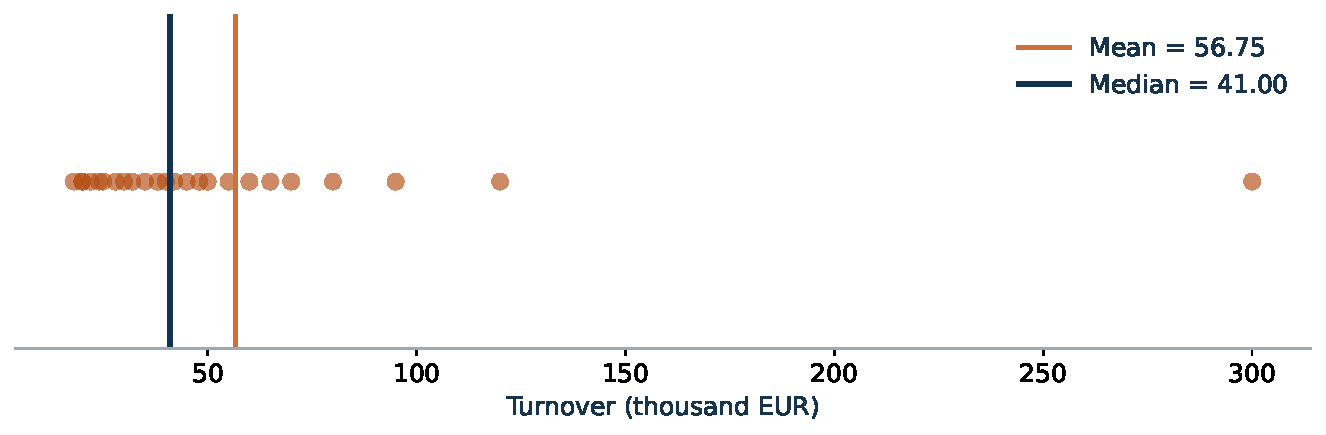
\includegraphics[width=\textwidth]{figures/centre.pdf}
An extreme value can be valid. Investigate its origin before deciding whether to exclude it.\\
Compare summaries with and without it, and document the decision.
\end{frame}

\begin{frame}{A weighted mean requires meaningful weights}
\[\bar{x}_w=\frac{\sum_i w_i x_i}{\sum_i w_i}.\]
Office A: 10 filings, 8 on time. Office B: 90 filings, 45 on time.
\begin{align*}
\text{Unweighted mean of office rates}&=(0.80+0.50)/2=0.65,\\
\text{Combined rate over filings}&=(8+45)/(10+90)=0.53.
\end{align*}
The first describes an average across the two offices. The second describes the 100 filings. The observational unit matters.
\end{frame}

\begin{frame}{Quantiles locate observations in an ordered distribution}
A quantile at probability $p$ describes a position in ordered data.\\
Sample quantile conventions can differ, especially for small datasets.
\par\vspace{2mm}
We use R's default, \texttt{type = 7}: let $h=1+(n-1)p$, $j=\lfloor h\rfloor$, $g=h-j$.
\[Q(p)=(1-g)x_{(j)}+g x_{(j+1)}\]
with the minimum and maximum at $p=0$ and $p=1$.
\par\vspace{2mm}
For turnover: $Q_1=27.25$, median $=41$, $Q_3=61.25$.\\
Thus $\operatorname{IQR}=Q_3-Q_1=34$ thousand EUR.
\source{R documentation: \href{https://stat.ethz.ch/R-manual/R-devel/library/stats/html/quantile.html}{Sample Quantiles}.}
\end{frame}

\begin{frame}{A boxplot is a compact summary}
The box spans $Q_1$ to $Q_3$, with the median marked inside.
\[\text{Lower fence}=Q_1-1.5\operatorname{IQR}\qquad
\text{Upper fence}=Q_3+1.5\operatorname{IQR}\]
Whiskers reach the most extreme observed values within the fences.\\
Observations outside the fences are shown separately.
\par\vspace{3mm}
Here the upper fence is $112.25$: turnovers 120 and 300 are flagged.\\
A flagged value is not automatically an error.
\source{The e-tivity uses type-7 quartiles. Base R boxplot hinges can differ from these quartiles.}
\end{frame}

\begin{frame}{Dispersion adds what a centre cannot show}
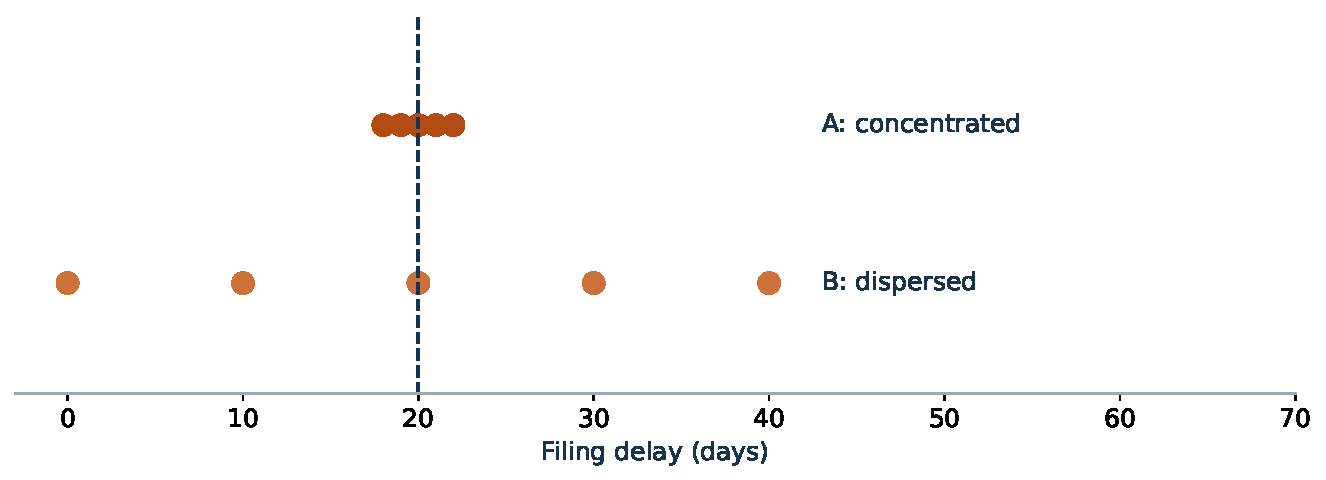
\includegraphics[width=\textwidth]{figures/spread.pdf}
Range $=\max(x)-\min(x)$. IQR $=Q_3-Q_1$.\\
The range depends on the endpoints. The IQR describes the middle part of the distribution.
\end{frame}

\begin{frame}{Why deviations cannot simply be added}
\[d_i=x_i-\bar{x},\qquad \sum_i d_i=0.\]
Positive and negative deviations cancel.
\par\vspace{3mm}
Two ways to summarise their magnitude are
\[\frac1n\sum_i|x_i-\bar{x}|\quad\text{and}\quad
\frac1n\sum_i(x_i-\bar{x})^2.\]
The first is the mean absolute deviation about the mean.\\
The second is the variance with denominator $n$.\\
Neither should be confused with the median absolute deviation (MAD).
\end{frame}

\begin{frame}{The variance denominator must be stated}
\begin{columns}[T]\column{.47\textwidth}\textbf{Describe the observed set}
\[v_n=\frac1n\sum_i(x_i-\bar{x})^2\]
This is the average squared deviation in these observations.
\column{.47\textwidth}\textbf{Estimate a population variance}
\[s^2=\frac1{n-1}\sum_i(x_i-\bar{x})^2\]
Under independent, identically distributed sampling with finite variance, this is an unbiased estimator of the population variance.
\end{columns}
\par\vspace{4mm}R's \texttt{var()} and \texttt{sd()} use $n-1$. Specify your convention. For $n=1$, the sample variance is undefined.
\end{frame}

\begin{frame}{Variance: a worked example}
\small
Processing times: $20,40,0,70$ days. Mean: $\bar x=32.5$ days.
\begin{center}\begin{tabular}{rrr}\toprule
$x_i$ & $x_i-\bar x$ & $(x_i-\bar x)^2$\\\midrule
20 & $-12.5$ & 156.25\\
40 & 7.5 & 56.25\\
0 & $-32.5$ & 1056.25\\
70 & 37.5 & 1406.25\\\midrule
 & Sum: 0 & Sum: 2675\\\bottomrule
\end{tabular}\end{center}
\[v_n=\frac{2675}{4}=668.75,\qquad s^2=\frac{2675}{3}\approx891.667.\]
Variance is in squared days. Sample SD: $s\approx29.861$ days.
\source{Values from the original Lecture 2 example, placed in an illustrative processing-time context. The e-tivity lets you change the fourth observation.}
\end{frame}

\begin{frame}{Standard deviation restores the original unit}
\[s=\sqrt{s^2}.\]
Turnover is measured in thousand EUR.\\
Variance is measured in squared thousand EUR.\\
Standard deviation is again measured in thousand EUR.
\par\vspace{3mm}
For the 24 firms, $s\approx57.73$ thousand EUR.\\
The large upper observation contributes strongly to this value.
\prompt{Why would a median and an IQR be useful alongside these summaries?}
\end{frame}

\begin{frame}{Changing units changes some summaries}
For $y_i=a+b x_i$:
\[\bar y=a+b\bar x,\qquad s_y=|b|s_x,\qquad s_y^2=b^2s_x^2.\]
Adding a constant moves the centre without changing the spread.\\
Multiplying by 1,000 converts thousand EUR into EUR and multiplies the standard deviation by 1,000.
\par\vspace{3mm}
\textbf{Coefficient of variation:}\quad $\mathrm{CV}=s/\bar{x}$.\\
Use it for positive ratio-scale measurements with a meaningful zero. A mean near zero makes it unstable. It is generally inappropriate for Celsius temperatures.
\end{frame}

\begin{frame}{E-tivity 2C: Heterogeneity and indices}
\Large Heterogeneity and indices\par\vspace{5mm}
\normalsize Complete the matching activity in the descriptive learning path.\par
\href{https://silviasaliniunimi.github.io/data-analysis-tax-compliance/02c-heterogeneity.html}{Open E-tivity 2C}\par

\end{frame}

\begin{frame}{Categorical heterogeneity is also variability}
For $K$ categories with proportions $p_1,\ldots,p_K$:
\[G=1-\sum_{j=1}^K p_j^2.\]
$G=0$ when every observation belongs to the same category.\\
For fixed $K$, the maximum is $1-1/K$, reached at equal proportions.
\par\vspace{3mm}
This is the \textbf{Gini--Simpson index} (also called Gini impurity).\\
It is different from the Gini coefficient of income inequality.\\
For sector counts $(12,8,4)$, $G\approx0.6111$.\\
Normalised: $G/(1-1/K)\approx0.9167$, with $K=3$.
\end{frame}

\begin{frame}{Entropy depends on the logarithm base}
\[H=-\sum_{j=1}^K p_j\log(p_j),\qquad 0\log 0:=0.\]
With natural logarithms: $0\leq H\leq\ln K$.\\
With base 2: the maximum is $\log_2 K$, in bits.\\
Unnormalised entropy can exceed 1.
\par\vspace{3mm}
For fixed $K>1$, $H/\log K$ lies between 0 and 1.\\
Use the same base in numerator and denominator.\\
For counts $(12,8,4)$: $H\approx1.0114$ nats and $H/\ln3\approx0.9206$.
\end{frame}

\begin{frame}{Category definitions change heterogeneity}
\textbf{Same units, a different classification}\\
Counts $(50,30,20)$ give $G=0.62$.\\
Splitting the last category into $(50,30,10,10)$ gives $G=0.64$.
\par\vspace{4mm}
The number and meaning of categories are part of the measurement. Normalisation does not make different classifications equivalent.
\par\vspace{4mm}
In classification trees, Gini impurity and entropy describe the mixture of outcome classes in a node. Sector diversity alone says little about compliance.
\source{Adapted from the supplied Heterogeneity Indices e-tivity.}
\end{frame}

\begin{frame}{A z-score is a relative position}
\[z_i=\frac{x_i-\bar{x}}s,\qquad s>0.\]
A value $z_i=1.5$ lies 1.5 sample standard deviations above the mean.\\
Positive $z$ means above the mean, not necessarily above the median.
\par\vspace{3mm}
Using the same complete observations and the sample SD gives
\[\bar z=0,\qquad s_z=1.\]
Standardisation does not make a skewed distribution normal.\\
If $s=0$, this z-score is undefined.
\end{frame}

\begin{frame}{Combining standardised variables requires a rationale}
Standardisation removes measurement units. It does not choose what matters.
\par\vspace{3mm}
An index such as $I_i=(z_{i1}+z_{i2})/2$ still requires decisions about:
\begin{itemize}
\item whether the variables measure the intended concept;
\item whether higher values have a consistent meaning;
\item whether equal weighting is justified;
\item how to handle missing values and correlated inputs.
\end{itemize}
A large index value is not, by itself, a validated risk assessment.
\end{frame}

\begin{frame}{A descriptive result needs an interpretation}
\textbf{Incomplete:}\quad ``The mean is 56.75.''
\par\vspace{3mm}
\textbf{Interpretable:}\\
``Across the 24 synthetic firms, mean turnover is 56.75 thousand EUR. The median is 41 thousand EUR, and the largest turnover is 300 thousand EUR. The upper tail raises the mean. These data do not estimate turnover in a real population.''
\par\vspace{3mm}
Report the variable, unit, observations, summary and scope of the conclusion.
\end{frame}

\begin{frame}[fragile]{The same definitions in R}
\begin{lstlisting}[language=R]
x <- d$turnover_kEUR
quantile(x, c(.25, .5, .75), type = 7)
c(mean = mean(x), sd = sd(x), IQR = IQR(x))
z <- as.numeric(scale(x))
p <- prop.table(table(d$sector))
G <- 1 - sum(p^2)
H <- -sum(p[p > 0] * log(p[p > 0]))
\end{lstlisting}
The supplied script also checks missing values and draws the graphs.
\end{frame}
\begin{frame}{Final self-check}
\begin{itemize}
\item Explain why a histogram with unequal bin widths needs density heights.
\item Interpret a mean, median, IQR and SD for the supplied turnover values.
\item State the ranges of Gini--Simpson and Shannon entropy.
\item Explain why missing audit outcomes cannot be treated as zero.
\item Explain what standardisation changes and what it preserves.
\end{itemize}
\end{frame}

\begin{frame}{Optional bridge: the Monty Hall experiment}
\small
Three doors: one car, two goats. The host knows where the car is, always opens an unchosen goat door and always offers a switch.
\begin{center}\begin{tabular}{lcll}\toprule
Initial choice & Probability & Stay & Switch\\\midrule
Car & $1/3$ & Win & Lose\\
Goat & $2/3$ & Lose & Win\\\bottomrule
\end{tabular}\end{center}
Repeated simulations produce observed proportions near $1/3$ and $2/3$. The probability model explains why.
\par\vspace{3mm}
The mechanism generating the information matters. We return to probability in the inference block.
\source{Condensed from the supplied Monty Hall e-tivity. This is an optional probability example, not a descriptive statistic or a taxpayer model.}
\end{frame}

\begin{frame}{Standardised components and their sum}
For standardised variables $Z_1,Z_2,Z_3$, each has sample mean 0 and sample variance 1 on the same observations.
\[\mathrm{Var}(Z_1+Z_2+Z_3)=3+2(r_{12}+r_{13}+r_{23}).\]
The sum has mean zero. Its standard deviation depends on the correlations.
\begin{itemize}
\item Uncorrelated components: SD $=\sqrt{3}$.
\item Identical standardised components: SD $=3$.
\end{itemize}
A positive z-score means above the mean. Z-scores have no universal bounds of $-3$ and $+3$.
\end{frame}
